%!TEX TS-program = xelatex
%!TEX encoding = UTF-8 Unicode

\documentclass[12pt]{extarticle}
% extarticle is like article but can handle 8pt, 9pt, 10pt, 11pt, 12pt, 14pt, 17pt, and 20pt text

\def \ititle {Origins of Mind}
 
\def \isubtitle {Lecture 08}
 
\def \iauthor {Stephen A. Butterfill}
\def \iemail{s.butterfill@warwick.ac.uk}
\date{}

%for strikethrough
\usepackage[normalem]{ulem}

\input{$HOME/Documents/submissions/preamble_steve_handout}

%logic symbol \leftmodels
\usepackage{MnSymbol}

%\bibpunct{}{}{,}{s}{}{,}  %use superscript TICS style bib
%remove hanging indent for TICS style bib
%TODO doesnt work
\setlength{\bibhang}{0em}
%\setlength{\bibsep}{0.5em}


%itemize bullet should be dash
\renewcommand{\labelitemi}{$-$}

\begin{document}

\raggedcolumns

\begin{multicols*}{3}

\setlength\footnotesep{1em}


\bibliographystyle{newapa} %apalike

%\maketitle
%\tableofcontents




%--------------- 
%--- start paste


\def \ititle {Logic I}
 
\def \isubtitle {Fast Lecture 05}
 
\begin{center}
 
{\Large
 
\textbf{\ititle}: \isubtitle
 
}
 
 
 
\iemail %
 
\end{center}
 
Readings refer to sections of the course textbook, \emph{Language, Proof and Logic}.
 
 
 
\section{Vegetarians Are Evil}
 
\emph{Reading:} §9.2, §9.3, §9.5
 
\begin{center}
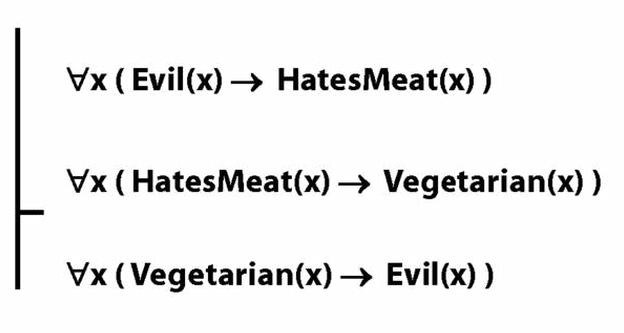
\includegraphics[scale=0.3]{img/vegetarians.png}
\end{center}
 
 
\section{Counterexamples with Quantifiers}
 
\begin{center}
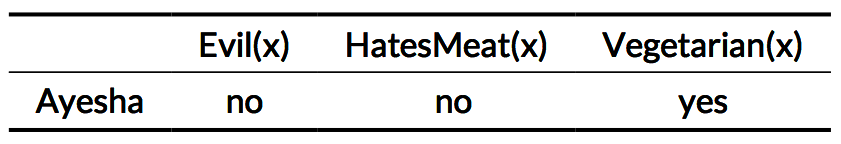
\includegraphics[scale=0.3]{img/unit_502b_counterexample.png}
\end{center}
 
 
\section{Something Is Above Something}
 
\emph{Reading:} §11.1
 
\begin{minipage}{\columnwidth}
 
Something is above something:
 
\hspace{3mm} ∃x ∃y Above(x,y)
 
\end{minipage}
 
 
 
\section{Multiple Quantifiers: Everyone Likes Puffins}
 
\emph{Reading:} §11.1
 
I like puffins:
 
\hspace{3mm} ∀x ( Puffin(x) → Likes(a,x) )
 
y likes puffins:
 
\hspace{3mm} ∀x ( Puffin(x) → Likes(y,x) )
 
Everyone likes puffins:
 
\hspace{3mm} ∀y ∀x ( Puffin(x) → Likes(y,x) )
 
 
 
\section{Relations: Transitivity}
 
\emph{Reading:} §15.1
 
A \emph{transitive} relation is one such that if x bears it to y and y bears it to z then x bears it to z. (E.g. LeftOf is transitive; NotAdjacent is not transitive.)
 
 
 \columnbreak
 
\section{Expressing Relations with Quantifiers}
 
\emph{Reading:} §15.1
 
\begin{minipage}{\columnwidth}
 
A \emph{reflexive} relation is one that everything bears to itself. (E.g. SameShape)
 
reflexive: ∀x R(x,x)
 
\begin{center}
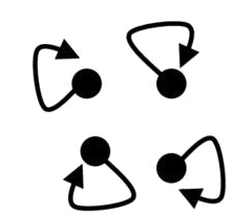
\includegraphics[scale=0.3]{img/reflexive.png}
\end{center}
\end{minipage}
 
\begin{minipage}{\columnwidth}
 
A \emph{symmetric} relation is one such that if x bears it to y, then y bears it to x. (E.g. Adjacent(x,y))
 
symmetric: ∀x∀y ( R(x,y) → R(y,x) )
 
\begin{center}

\includegraphics[scale=0.3]{img/symmetric.png}
\end{center}
\end{minipage}
 
\begin{minipage}{\columnwidth}
 
A \emph{transitive} relation is one such that if x bears it to y and y bears it to z then x bears it to z. (E.g. LeftOf is transitive; DifferentShape is not transitive)
 
transitive: ∀x∀y∀z ( ( R(x,y) ∧ R(y,z) ) → R(x,z) )
 
\begin{center}
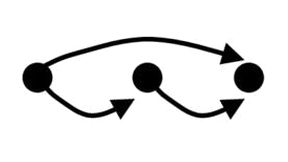
\includegraphics[scale=0.3]{img/transitive.png}
\end{center}
\end{minipage}
 
 
 
\section{Expressing Counterexamples Formally}
 
\emph{Reading:} §15.1
 
Give a counterexample to this argument:
 
\begin{center}
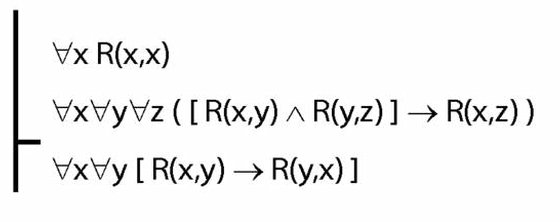
\includegraphics[scale=0.3]{img/unit_583_argument.png}
\end{center}
Informally:
 
\begin{center}
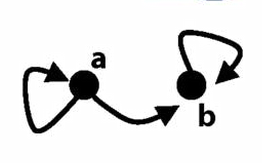
\includegraphics[scale=0.3]{img/unit_583_counterexample.png}
\end{center}

Formally:

\hspace{3mm} Domain: \{a, b\}
 
\hspace{3mm} R: \{<a,a>, <a,b>, <b,b>\}
 
 
 
\section{There Is a Store for Everything}
 
\emph{Reading:} §11.2, §11.3
 
There is a store for everything:
 
\hspace{3mm}	∃y∀x StoreFor(y,x)
 
\hspace{3mm} ∀y∃x StoreFor(x,y)
 
Other sentences to translate:
 
\hspace{3mm} Wikipedia has an article about everything
 
\hspace{3mm} Everyone hurts someone they love
 
\hspace{3mm} Someone hurts everyone she loves
 
 
 
\section{∀Intro: An Incorrect Proof}
 
\emph{Reading:} §13.1, §13.2
 
This proof is wrong, but why?:
 
\begin{center}
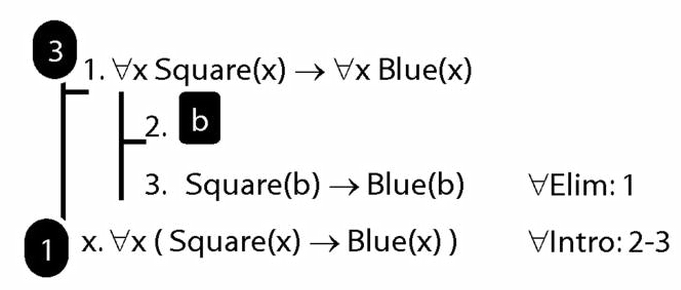
\includegraphics[scale=0.3]{img/unit_572_proof.png}
\end{center}
There is a counterexample to the argument:
 
\begin{center}
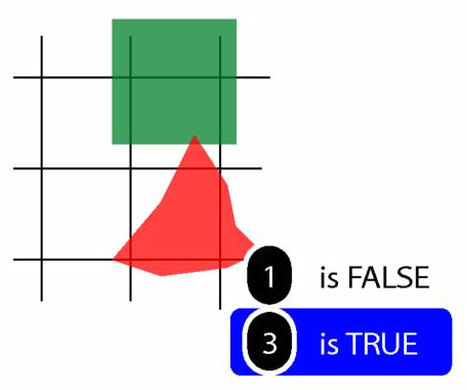
\includegraphics[scale=0.3]{img/unit_572_proof2.png}
\end{center}
 
\columnbreak
 
\section{Two Things Are Broken}
 
\emph{Reading:} §14.1
 
To translate sentences involving number into FOL, use identity. For example,
 
`Two things are broken' might be translated as:
 
∃x ∃y ( Broken(x) ∧ Broken(y) ∧ ¬(x=y) )
 
 
 
\section{Quantifier Equivalences: \\ ∀x(Square(x) → Broken(x)) $\leftmodels\models$ ∀x(¬Broken(x) → ¬Square(x))}
 
\emph{Reading:} §10.3
 
\begin{center}
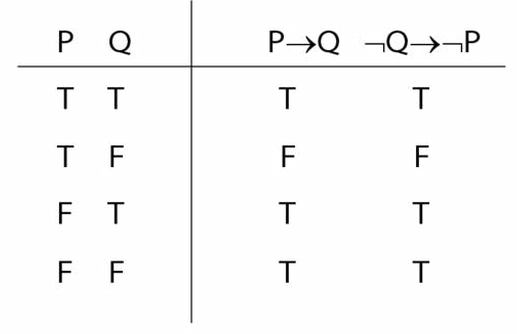
\includegraphics[scale=0.3]{img/unit_760_tt.png}
\end{center}
 
 
\section{Quantifier Equivalences: \\ ∀x Created(x) $\leftmodels\models$ ¬∃x Created(x)}
 
\emph{Reading:} §10.3, §10.4
 
 
 \columnbreak
\section{Soundness and Completeness: Statement of the Theorems}
 
\emph{Reading:} §8.3, §13.4
 
‘A $\vdash$ B’ means there is a proof of B using premises A
 
‘$\vdash$ B’ means there is a proof of B using no premises
 
‘A $\models$ B’ means B is a logical consequence of A
 
‘$\models$ B’ means B is a tautology
 
‘A $\models$$_{TT}$ B’ means B is a logical consequence of A just in virtue of the meanings of truth-functions (the textbook LPL calls this ‘tautological consequence’)
 
\emph{Soundness}: If A $\vdash$ B then A $\models$ B
 
\hspace{3mm} i.e. if you can prove it in Fitch, it’s valid
 
\emph{Completeness}: If A $\models$$_{TT}$ B then A $\vdash$ B
 
\hspace{3mm} i.e. if it’s valid just in virtue of the meanings of the truth-functional connectives, then you can prove it in Fitch.
 


%--- end paste
%--------------- 
 

\end{multicols*}

\end{document}